Las pruebas que serán mostradas en este último capítulo, corresponden a una demostración funcional del sistema web.
Se demostrará que los requisitos funcionales descritos en el Capítulo \ref{Desarrollo_Sistema} se cumplan.
\subsection{REQF-01: Autentificación de usuario}


En la Figura \ref{REQF-01} se muestra el inicio de sesión, los campos son: R.U.N del usuario y
Contraseña,


	\begin{figure}[H]
		\centering
		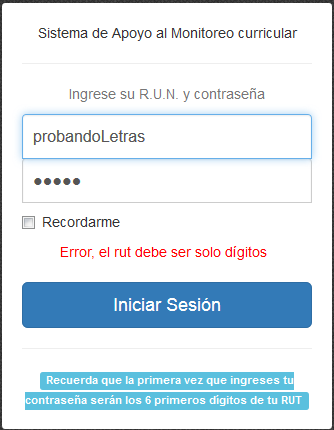
\includegraphics[width=0.5\textwidth]{images/Capitulo_5/REQF-01.png}
		\caption[REQF-01: Autentificación de usuario]{REQF-01: Autentificación de usuario \footnote{}}
		\label{REQF-01}
	\end{figure}
	\footnotetext{Elaboración propia.}
	
	
	Se realizaron distintas pruebas para comprobar el correcto funcionamiento de este requisito. A continuación se describen las distintas pruebas realizadas:
	\begin{itemize}
		\item Validación de números: El nick del usuario es su R.U.N. sin el dígito verificador, por lo que el sistema tiene que validar si el usuario ingresa cualquier carácter que no corresponda a un dígito. En caso de que el usuario ingrese algún carácter que no sea dígito, el sistema muestra el siguiente mensaje: \textbf{Error, el rut debe ser solo dígitos.}
		
		\item Validación nula: Los  dos campos solicitados  este formulario son campos obligatorios, por lo que si el usuario hace click en iniciar sesión y no ha completado estos campos, el sistema muestra un mensaje de alerta, impidiendo que el servidor realice cálculos innecesarios. Esta validación se ilustra en la Figura \ref{REQF-01-null}.
	\end{itemize}
	
	\begin{figure}[H]
		\centering
		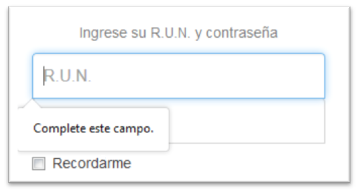
\includegraphics[width=0.7\textwidth]{images/Capitulo_5/REQF-01-null.png}
		\caption[REQF-01: Autentificación de usuario, validación de campos nulos]{REQF-01: Autentificación de usuario, validación de campos nulos}
		\label{REQF-01-null}
	\end{figure}
	
\subsection{REQF-02: Gestión de perfil}

\begin{figure}[H]
	\centering
	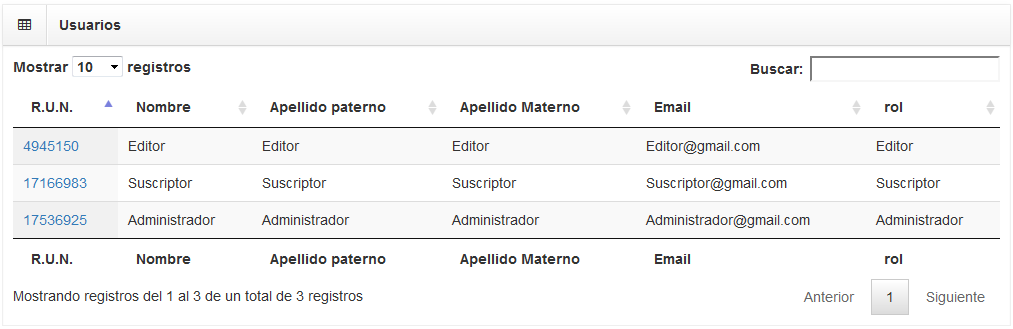
\includegraphics[width=1\textwidth]{images/Capitulo_5/REQF-02.png}
	\caption[REQF-02: Gestión de perfil]{REQF-02: Gestión de perfil}
	\label{REQF-02}
\end{figure}

La Figura \ref{REQF-02} ilustra la gestión de perfiles del sistema,  este requerimiento solo puede ser accedido por un usuario de tipo administrador.
\\
En primer lugar se realizaron pruebas para comprobar que los usuarios del tipo Editor y Suscriptor  no tuvieran acceso, para ello se crearon  tres usuarios con los tres tipos de perfiles existentes, con el fin de autentificarse y tratar de acceder a este requisito. los resultados muestran en la Tabla \ref{pruebas_gestionPerfiles}.

\newpage
	\begin{longtable}{l |l}
		
		\caption{Resultados de pruebas del acceso a la gestión de perfiles}
		\label{pruebas_gestionPerfiles}\\
		
		
		\hline
		\endfirsthead
		\multicolumn{2}{c}%
		{\tablename\ \thetable\ -- \textit{Continuación de la pagina anterior}} \\
		\hline
		
		\hline
		\endhead
		\hline \multicolumn{2}{r}{\textit{Continúa en la página siguiente}} \\
		\endfoot
		\hline
		\endlastfoot
		\rowcolor{LightBlue2} Tipo de perfil & Resultado de acceso\\ \hline
		
		Administrador & Se pudo acceder exitosamente.\\ \hline
		
		Editor & No se pudo acceder.\\ \hline
		
		Suscriptor & No se pudo acceder.\\ \hline \hline
	\end{longtable}

En segundo lugar se realizaron pruebas para las siguientes operaciones básicas de este requisito: Actualizar usuario y Eliminar usuario. el proceso y los resultados de cada prueba se detallan a continuación.

\mysubparagraph{Actualizar usuario}

Uno de los Errores encontrados al momento de validar esta acción, fue que al tratar de actualizar  un usuario en particular  los datos que se enviaban mediante la petición POST al servidor no eran los correctos. El error detectado se puede apreciar gráficamente en las Figuras \ref{REQF-02-actualizar} y \ref{REQF-02-post}.


\begin{figure}[H]
	\centering
	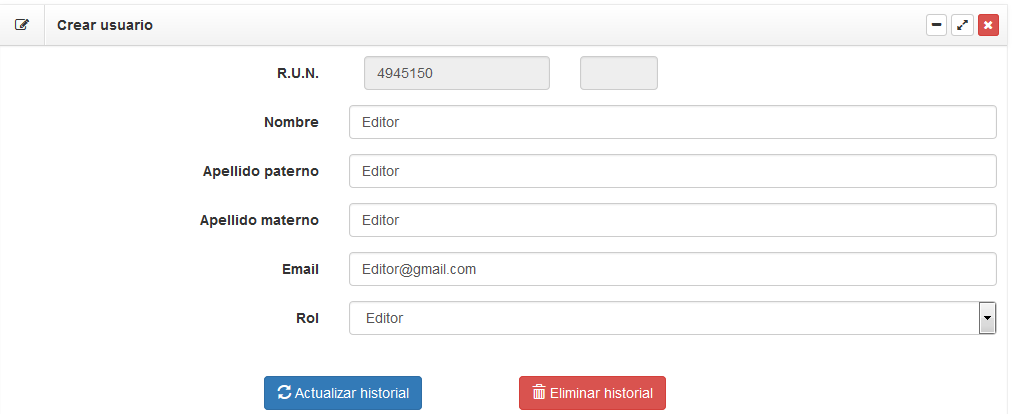
\includegraphics[width=1\textwidth]{images/Capitulo_5/REQF-02-agregar1.png}
	\caption[REQF-02: Gestión de perfil, Actualizar usuarios]{REQF-02: Gestión de perfil, Actualizar usuarios}
	\label{REQF-02-actualizar}
\end{figure}

Aunque el usuario autentificado esta intentando editar el  R.U.N. 4.945.150, en la Figura \ref{REQF-02-post}  se puede apreciar que, entre las variables que se están enviando, esta la variable Rut, que corresponde al R.U.N. editado, sin embargo el valor que esta tomando la variable  Rut no corresponde al R.U.N. editado, si no  que se esta enviando el R.U.N. de la persona autentificada. Este error fue corregido a tiempo.
\begin{figure}[H]
	\centering
	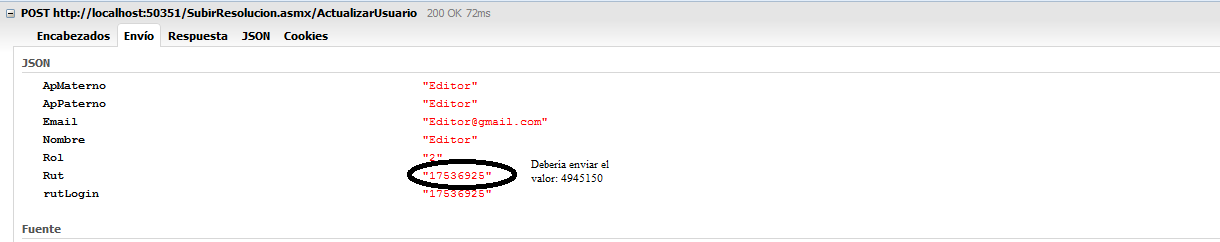
\includegraphics[width=1\textwidth]{images/Capitulo_5/REQF-02-post.png}
	\caption[REQF-02: Gestión de perfil, depuración de los datos enviados mediante la petición POST]{REQF-02: Gestión de perfi, depuración de los datos enviados mediante la petición POST}
	\label{REQF-02-post}
\end{figure}

\mysubparagraph{Eliminar usuario}

Comprobar el correcto funcionamiento del mensaje de alerta que se muestra en la Figura \ref{REQF-02-eliminar} era el principal objetivo de la validación de esta acción, ya que como se mencionó en la Sección \ref{Dificultades}, ASP.NET trabaja de una forma particular las peticiones POST de complementos externos.
\begin{figure}[H]
	\centering
	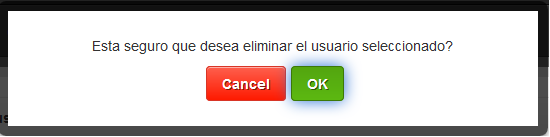
\includegraphics[width=1\textwidth]{images/Capitulo_5/REQF-02-Eliminar.png}
	\caption[REQF-02: Gestión de perfil, Mensaje de verificación para eliminar algún usuario]{REQF-02: Gestión de perfi, Mensaje de verificación para eliminar algún usuario}
	\label{REQF-02-eliminar}
\end{figure}

La acción eliminar usuario no presentó mayores problemas.


\subsection{REQF-03: Desplegar historial curricular}

Este requerimiento no necesitó mayores pruebas puesto que es un requerimiento de visualización.

\subsection{REQF-04: Registro de usuarios}

Uno de los datos que NO se pueden modificar una vez que se haya creado el usuario, es el R.U.N., por lo que es de vital importancia que este dato se ingrese correctamente al momento de ingresar el usuario, para ello se consideró validar la existencia del R.U.N. ingresado mediante el plugins jQuery.Rut.js. \\

En caso de que el R.U.N. ingresado no existiera el sistema muestra gráficamente un mensaje de que el R.U.N. no existe (Ver Figura \ref{REQF-02-rut}), impidiendo que el usuario se almacene en la base de datos.

\begin{figure}[H]
	\centering
	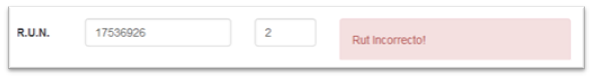
\includegraphics[width=1\textwidth]{images/Capitulo_5/REQF-02-rut.png}
	\caption[REQF-02: Gestión de perfil]{REQF-02: Gestión de perfil}
	\label{REQF-02-rut}
\end{figure}

Con respecto a los demás campos se validó que todos los campos sean obligatorios y que el formato del correo electrónico sea un formato  válido.


\subsection{REQF-05:Gestión de documentos}

Se realizaron distintas pruebas para comprobar el correcto funcionamiento de este requisito. A continuación se describen las distintas pruebas realizadas:
\begin{itemize}
	\item Validación nula: Todos los  campos solicitados en  este formulario son campos obligatorios, por lo que si el usuario deja un campo sin completar, y luego  hace click en Subir archivos, el sistema de forma inmediata marca en rojo todos los campos que no se han completado, y le informa al usuario de que son campos obligatorios.
	
	\item Validación de Formato de archivos: Se intentó subir archivos de distintos formatos (.jpg, word, ppt, etc) y el resultado que el sistema muestra un mensaje de Alerta indicando que el formato no es el correcto (Ver Figura \ref{REQF-05} ).
	
	\item Validación de eliminación de archivos: Se eliminaron registros curriculares con el fin de verificar que el registro se eliminara en su totalidad del sistema, es decir, que se eliminaran el registro en la base de dato y que se eliminara los archivos vinculados a ese registro eliminado del servidor.
\end{itemize}


\begin{figure}[H]
	\centering
	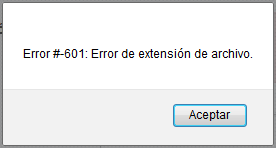
\includegraphics[width=0.5\textwidth]{images/Capitulo_5/REQF-05.png}
	\caption[REQF-05: Gestión de documentos, Mensaje de alerta ]{REQF-05: Gestión de documentos, Mensaje de alerta }
	\label{REQF-05}
\end{figure}
\subsection{REQF-06:Visor de PDF}

Se realizaron distintas pruebas para comprobar el correcto funcionamiento de este requisito. A continuación se describen las distintas pruebas realizadas:

\subsection{REQF-07:Notificaciones}


El sistema de notificaciones esta presente en todo el sistema, por lo que este requerimiento  fue validado a medida que se fueron validando los demás  requisitos, en la Figura \ref{REQF-07} se muestra un ejemplo de una notificación exitosa.
 
\begin{figure}[H]
	\centering
	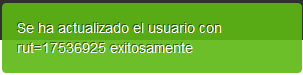
\includegraphics[width=0.5\textwidth]{images/Capitulo_5/REQF-07.png}
	\caption[REQF-07: Notificaciones, alerta exitosa ]{REQF-07: Notificaciones,alerta exitosa }
	\label{REQF-07}
\end{figure}



\subsection{REQF-08:Almacenar bitácora de los usuarios}


El objetivo de este requisito es tener un control y un historial de todas las notificaciones de los eventos ocurridos en la plataforma.
Este requerimiento utiliza las salidas de los procedimientos y los servicios para posteriormente almacenarlos en una tabla de la base de datos.


Es de vital importancia que este requisito funcione en su totalidad, ya que es el encargado de registrar todos los eventos de todos los otros requisitos.


depende mucho de las salidas de los procedimientos y de las salidas de los servicios


En principio este requisito surgió en la última iteración del proyecto,  por lo que fue una de las validaciones más complicadas y de las que demandó más tiempo, ya que, y


La validación de este requisito fue muy distinta   a las otras validaciones del sistema, ya que las validaciones anteriores se hicieron sobre la plataforma y los resultados se visualizaban sobre el sistema, por el contrario esta validación se tuvo que realizar depurando la aplicación web.\\

Hay que mencionar que este requisito surgió en la iteración final del proyecto, por lo que la mayoría de los procedimientos y servicios web ya estaban programados y esto ocasionó que la depuración de la plataforma sea engorrosa.
\\

En primer lugar se hizo una validación de los procedimientos de la base de datos, con el objetivo de que todos los procedimientos tengan una salida estándar y así poder tener un formato de los eventos ocurridos en el sistema.
\\





Este fue uno de los requerimientos que surgió en la última iteración, por lo que fue una de las validaciones más complicadas y de las que demandó más tiempo, razón por la cual los eventos no poseían un formato definitivo de cómo se almacenarían los datos.
\\

Se realizaron distintas pruebas para comprobar el correcto funcionamiento de este requisito. A continuación se describen las distintas pruebas realizadas:

\begin{itemize}
	\item validación salida de procedimientos:En un principio los procesos almacenados de la base de datos no poseían una salida estándar, por lo que el primer paso para lograr con éxito este requerimiento, fue reprogramar todos los procedimientos almacenados y validar de que todos tuvieran la misma salida.
	
	\item validación salida de los servicios web: al igual que en los procedimientos almacenados, los servicios web se tuvieron que estandarizar y verificar mediante la consola de Firefox el retorno de éstos servicios.
\end{itemize}





El proceso de validación de este requerimiento comenzó validando el mensaje de salida de los procedimientos almacenados de la base de datos, el cual no fue fácil ya que como en un principio este requerimiento no existía, los procedimientos no tenían una salida estándar,


\subsection{REQF-09:Visualización de bitácora}

Este requerimiento no necesitó mayores pruebas puesto que es un requerimiento de visualización.
